\begin{figure*}[!htb]
        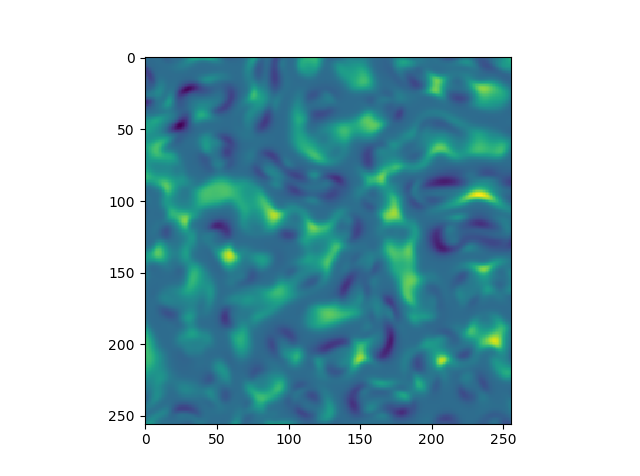
\includegraphics[width=0.33\linewidth]{img/dataset/miranda-viscosity.png}
        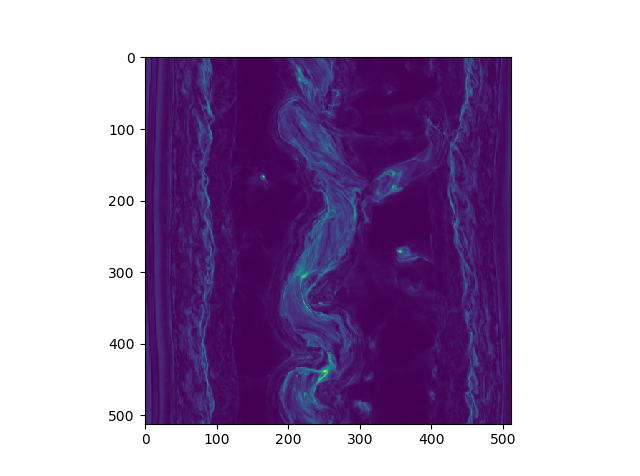
\includegraphics[width=0.33\linewidth]{img/dataset/magnetic.png}
        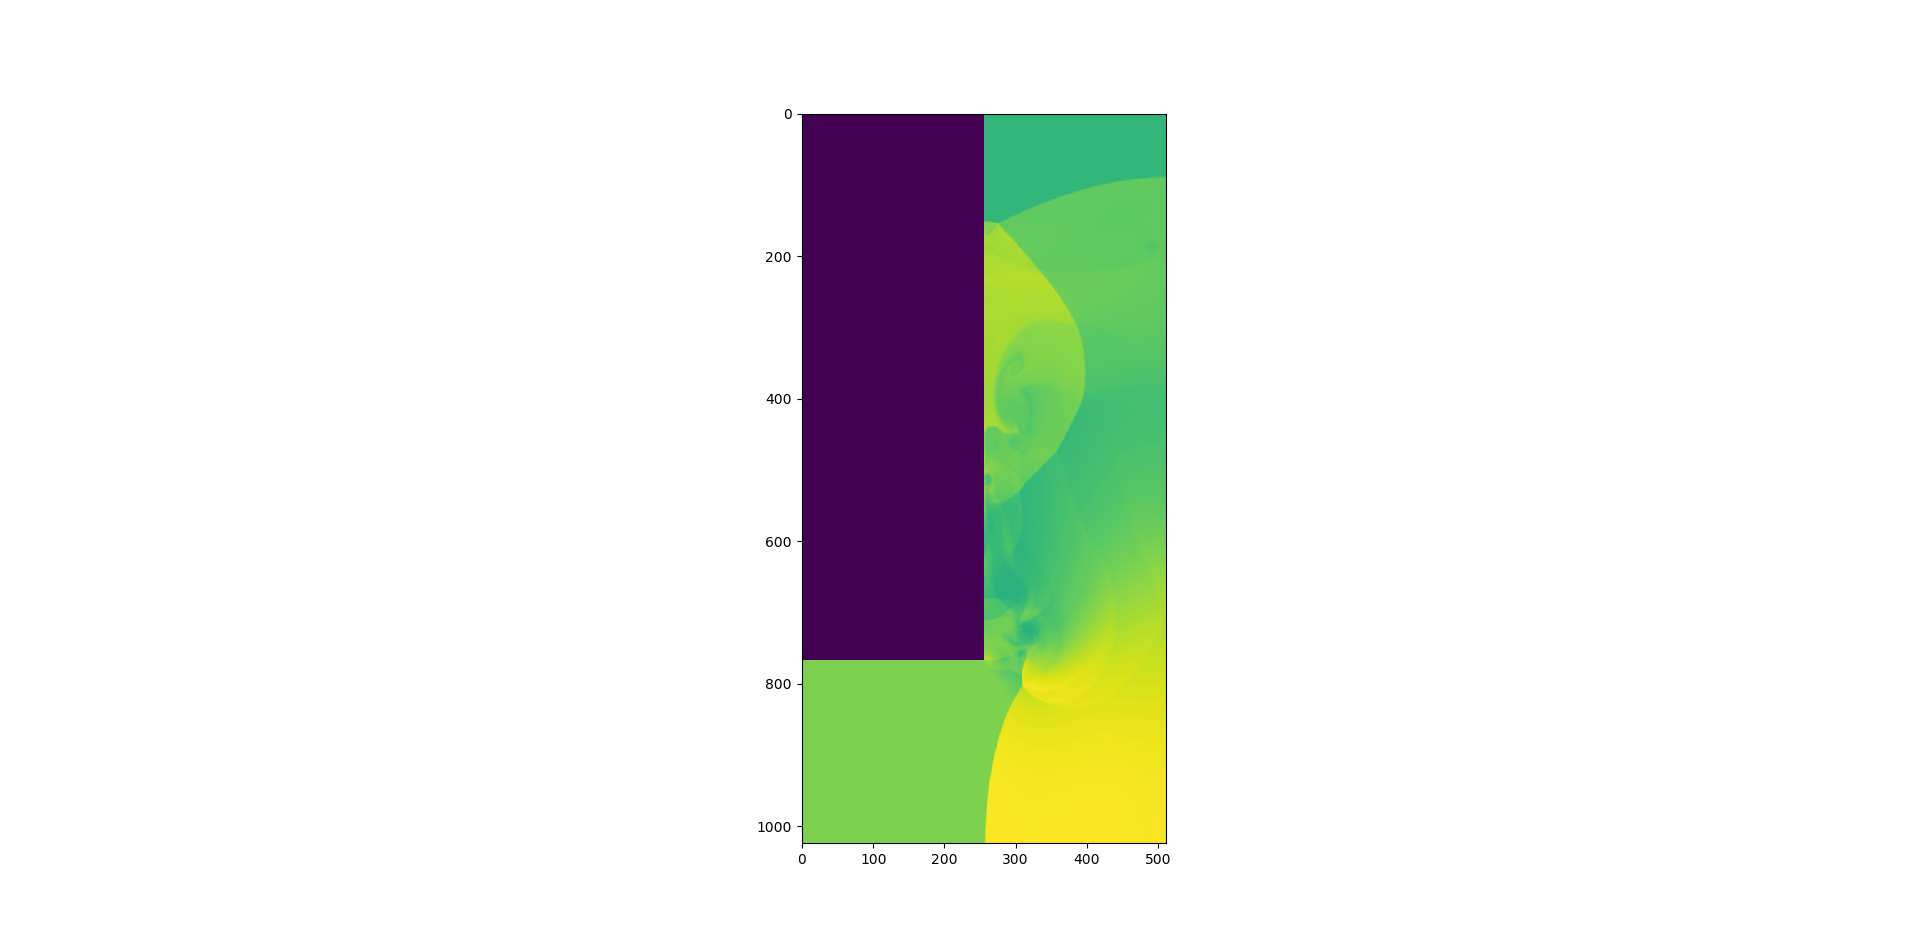
\includegraphics[width=0.33\linewidth]{img/dataset/euler2d.png}
        \caption{Left to right: miranda viscosity field, magnetic reconnection, euler 2d sharp front}
        \label{fig:datasets}
\end{figure*}

\section{The need for fine-granularity streams}
Multiresolution data structures or value quantization are commmonly used for data size
reduction.

However, we show that by both reducing resolution and precision we can achieve lower error
than by limiting the reduction only to resolution or only to precision. For our experiments
we use wavelets, where the resolution corresponds to levels, and precision to bitplanes.

For example, we can compute {\em PSNR} for a relatively smooth and uniform dataset, such as Miranda
viscosity field, and vary only resolution, only precision, or both (\Cref{fig:psnr_traditional_vs_by_norm_viscosity}). Miranda
dataset is especially useful as the independent stream order does not exhibit any spatial adaptivity and
this particular datasets is fairly uniform.

\begin{figure}[htb!]
	\centering
	\subcaptionbox{without skip leading zeros}
	{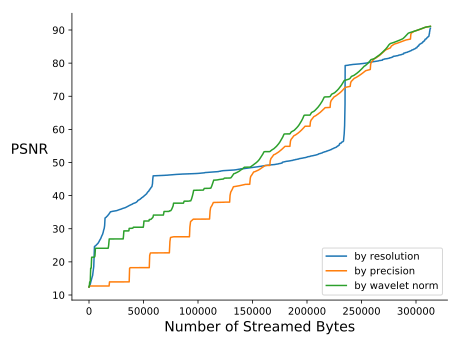
\includegraphics[width=0.4\linewidth]{img/independent/rmse-miranda-viscosity}}
	\subcaptionbox{with skip leading zeros}
	{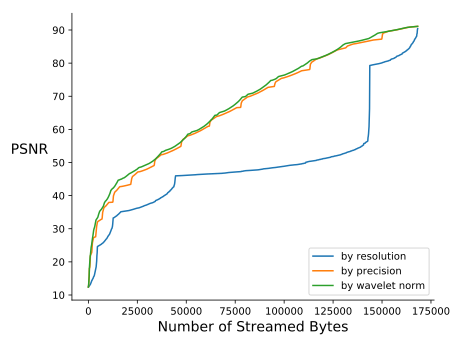
\includegraphics[width=0.4\linewidth]{img/skip-zeros/rmse-miranda-viscosity}}
	\caption {PSNR comparison between three streams: by bit-plane, by level, and by wavelet norm}
	\label{fig:psnr_traditional_vs_by_norm_viscosity}
\end{figure}



The resolution stream loads level-by-level data with full precision resulting in notable flat regions. These
regions are coused by the doubling of the samples at each refinement step. Similarly, the precision stream
shows the similar staircase pattern, but in this case the flat regions are smaller as the bitplane granularity
is finer than in the resolution stream case. The combination of both these approaches outperform precision
stream at all times and its finer granularity.

We begin by defining what we mean by resolution and precision. Things to touch on here:

\begin{enumerate}
  \item that we use the (cdf5/3) wavelet transform to generate levels of resolution (subbands)
  \item that due to computational contraint, and also because of practical reasons, we group wavelet coefficients into groups of 4x4 (and in some cases 8x8 or 16x16 if the data is large).
  \item we quantize the data to 16 bits by extracting the maximum exponent
  \item we use negabinary to avoid having to deal with the sign bit in a special way
\end{enumerate}

Here we argue that streaming by bit planes or streaming by levels result in sub-optimal PSNR (\Cref{fig:psnr_traditional_vs_by_norm_viscosity}a)


When compression is used, it avoids streaming the leading zero bits of the wavelet coefficients (figure \ref{fig:psnr_traditional_vs_by_norm_viscosity}b).

In the supplement materials, we show the same plot for the following datasets:
\begin{enumerate}
  \item Miranda viscosity (smooth and uniform)
  \item Kingsnake (noisy and sparse)
  \item Magnetic (tiny narrow lines)
  \item Euler 2D (sharp front)
  \item Enzo u (wide range)
\end{enumerate}

The reader may ask: if I already have a good, practical PSNR stream (the data-independent, by bit plane, skip leading zeros), why do I need other streams? Here we show that for isocontour extraction, and for histogram computation, we are better off with other streams.
  
Figure: isocontour error for the same data set (Figure \ref{fig:by_bit_plane_isocontour})
\begin{enumerate}
  \item Data-dependent stream for isocontour with skip leading zeros
  \item Data-dependent stream for isocontour with skip leading zeros, also with by-bit-plane constraint
\end{enumerate}

We also need to show a rendering of the two isocontours for these streams at some low bit rate.

\begin{figure}[htb!]
	\centering
	\subcaptionbox{without skip leading zeros}
	{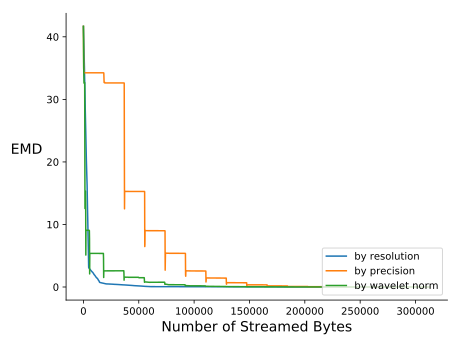
\includegraphics[width=0.4\linewidth]{img/independent/histogram-miranda-viscosity}}
	\subcaptionbox{with skip leading zeros}
	{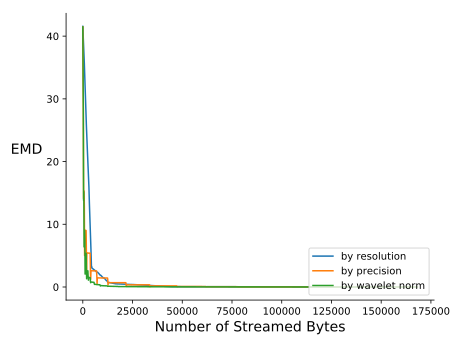
\includegraphics[width=0.4\linewidth]{img/skip-zeros/histogram-miranda-viscosity}}
	\caption {Histogram with earth mover distance (EMD) comparison between three streams: by bit-plane, by level, and by wavelet norm}
	\label{fig:histogram_traditional_vs_by_norm_viscosity}
\end{figure}



\begin{enumerate}
  \item Data-dependent stream for histogram with skip leading zeros
  \item Data-dependent stream for histogram with skip leading zeros, also with by-bit-plane constraint
\end{enumerate}  
  Here we also show renderings of different histograms corresponding to the different streams at some low bit rate.

\begin{figure}
  \centering
  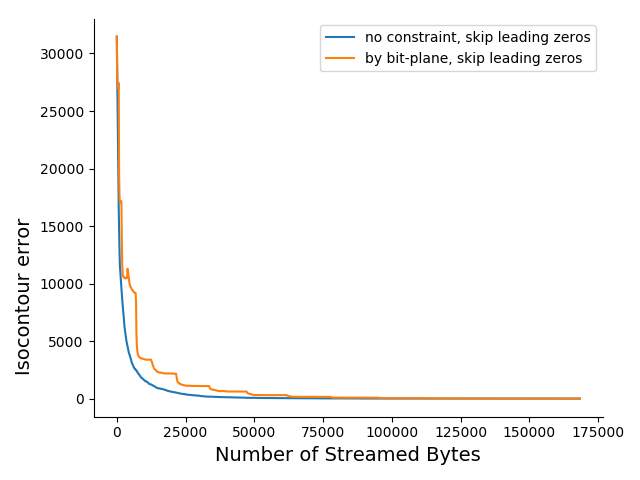
\includegraphics[width=0.8\linewidth]{resources/isocontour-error-by-bit-plane-viscosity.png}
  \caption {By bit-plane isocontour comparison versus no constraints for viscosity, isoval=-0.005}
  \label{fig:by_bit_plane_isocontour}
\end{figure}
